\documentclass[10pt]{beamer} 
\usepackage{lmodern}
\setbeamertemplate{footline}[frame number]
\usepackage{graphicx}



\title{Domača Naloga 1}
\author{Miha Kokalj, 23221209}
\institute{Fakulteta za strojništvo, Univerza v Ljubljani} 
\date{7.11.2024} 
\begin{document} 
\frame{\titlepage}

\begin{frame}
\frametitle{Kazalo}
 \tableofcontents[sectionstyle=show, subsectionstyle=show]
 
\end{frame}

\section{Vsebina datoteke}
\begin{frame}
\frametitle{Vsebina datoteke}
Podatki predstavljajo časovne korake v katerih smo merili moč P[W]
\begin{itemize}
    \item Prva vrstica datoteke : Čas [s]
    \item Druga vrstica datoteke : Število vrstic in število podatkov v vrstici
\end{itemize}

\vspace{5pt}
Za branje podatkov iz datoteke sem uporabil funkcijo \textbf{importdata} :
\begin{itemize}
    \item \textbf{importdata}: Prebere vsebino datoteke in vrne strukturo ali numerično matriko, odvisno od oblike podatkov v datoteki.  
\item \textbf{data.data}: Iz strukture, ki jo vrne `importdata`, izlušči samo numerične podatke.
    \item Kot izhod dobimo podatke, shranjene v vektor.
\end{itemize}
\end{frame}

\section{Graf P(t)}
\begin{frame}
\frametitle{Graf P(t)}
\begin{figure}
    \centering
    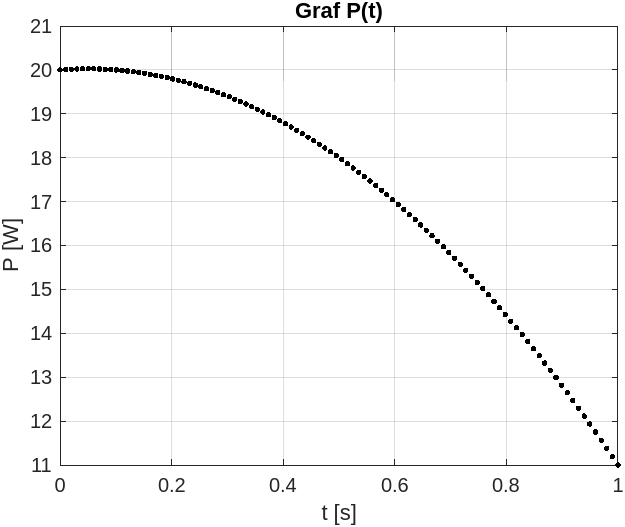
\includegraphics[width=0.8\textwidth]{graf_P(t).png} 
    \caption{Prikaz grafa \( P(t) \): moč v odvisnosti od časa.}
    \label{fig:P_t}
\end{figure}
\end{frame}

\section{Trapezna metoda}
\begin{frame}[fragile]
\frametitle{Trapezna formula}
\begin{itemize}
    \item Za približen izračun ploščine pod grafom \( P(t) \), sem uporabil trapezno formulo:
    \[
    \int_{t_{\text{min}}}^{t_{\text{max}}} P \, dt \approx \sum_{i=1}^{n-1} \frac{h_i}{2} (P_i + P_{i+1}),
    \]
    kjer je \( h_i = t_{i+1} - t_i \) časovni korak.
    
    \item Formula je bila implementirana v MATLAB s pomočjo zanke \textbf{for}:
\begin{verbatim}
vrednost_integrala = 0
dt = t(2) - t(1); 
for i = 1:length(P)-1
    vrednost_integrala = vrednost_integrala + (P(i) + P(i+1)) * dt / 2;
end
\end{verbatim}
    \item \textbf{Rezultat izračuna:} \( 17.1665 \, \text{J} \)
\end{itemize}
\end{frame}



\end{document}